\section{Autentifikacija korisnika}

\subsection{Početni zaslon}

\begin{figure}[H]
  \centering
  \includegraphics[width=0.35\textwidth]{images/implementacija/first.png}
  \caption{Početni zaslon mobilne aplikacije "Alpinity"}
  \label{fig:prvi_zaslon}
\end{figure}

Prvi korak u korištenju aplikacije "Alpinity" je početni zaslon koji služi kao ulazna točka u mobilnu aplikaciju (slika~\ref{fig:prvi_zaslon}). Ovaj zaslon nudi tri opcije, prijavu, registraciju i pristup izvanmrežnom načinu rada (eng. \textit{offline mode}).

\begin{figure}[H]
  \centering
  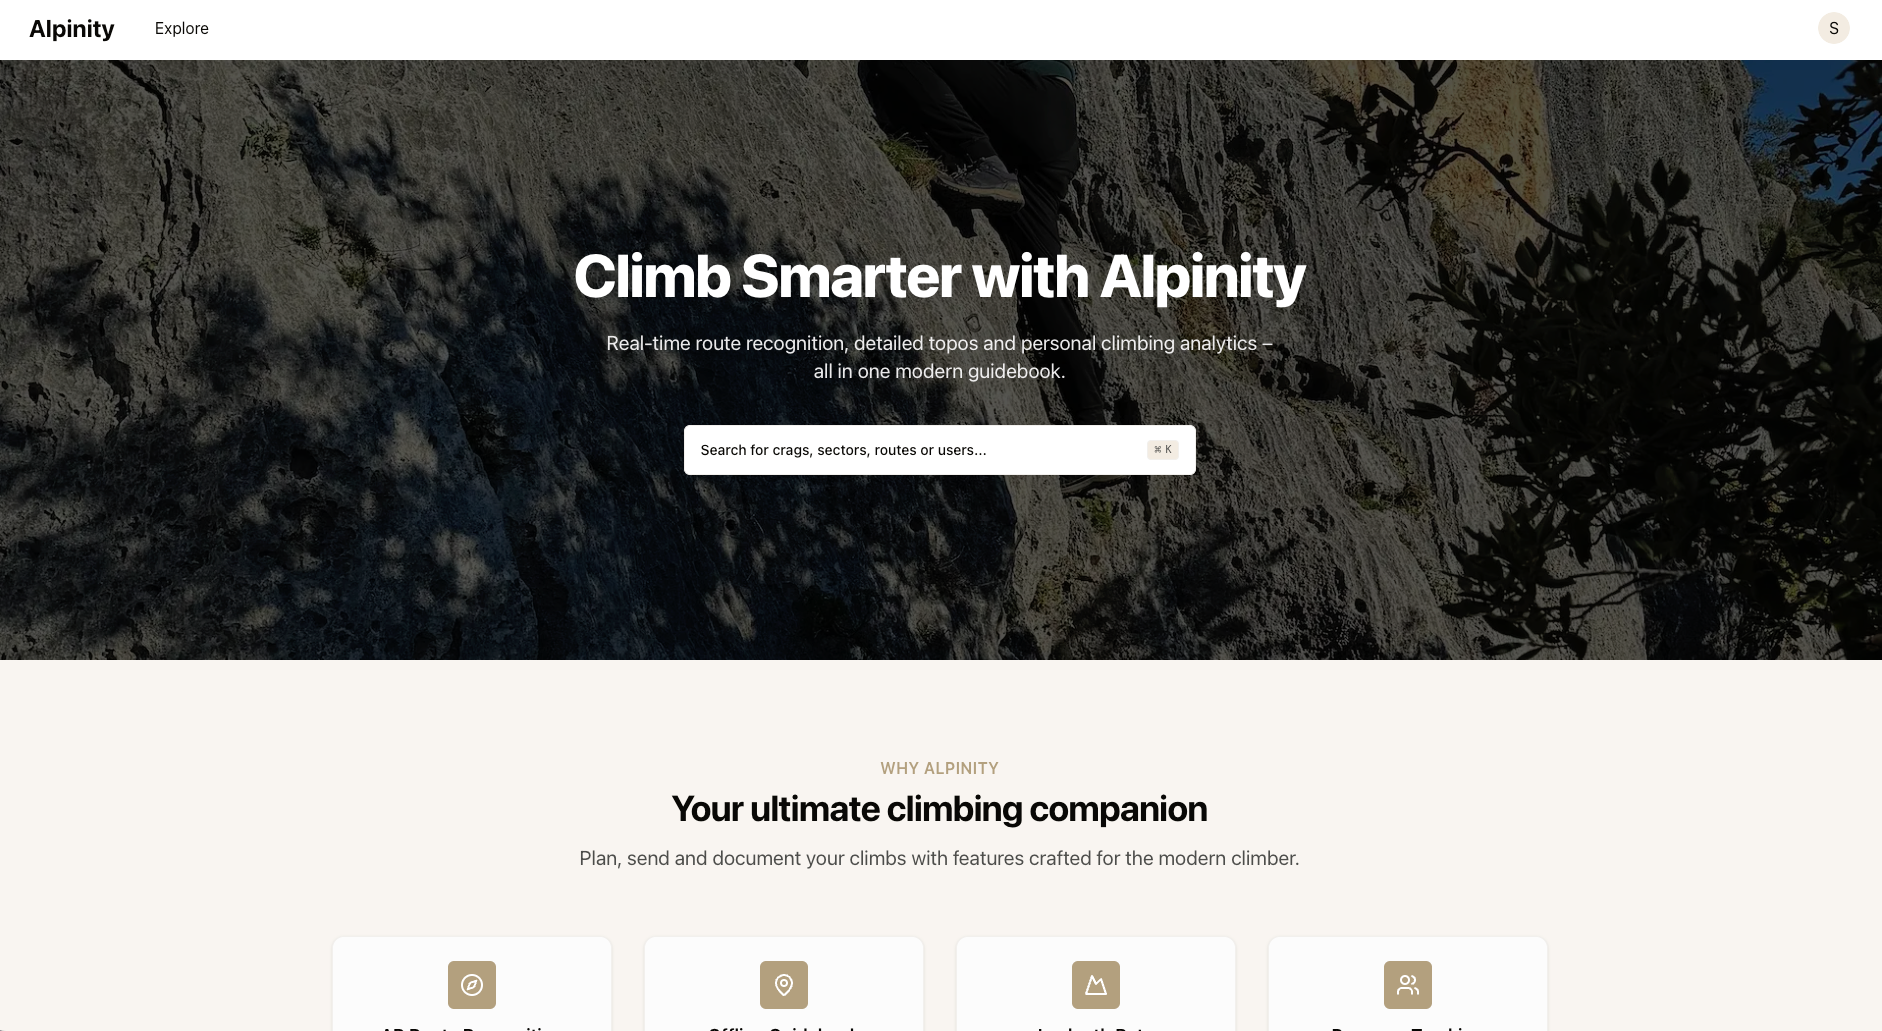
\includegraphics[width=0.9\textwidth]{images/implementacija/web/pocetni_zaslon.png}
  \caption{Početni zaslon web aplikacije "Alpinity"}
  \label{fig:prvi_zaslon_web}
\end{figure}

Na web aplikaciji, korisniku se prikazuje početni zaslon koji sadrži opis funkcionalnosti aplikacije (slika~\ref{fig:prvi_zaslon_web}). U gornjem desnom kutu nalazi se gumb za prijavu koji vodi na stranicu za prijavu iz koje se može odabrati opcija za registraciju.

\subsection{Registracija korisnika}

\begin{figure}[H]
  \centering
  \begin{subfigure}{.5\textwidth}
    \centering
    
\includegraphics[width=0.7\linewidth]{images/implementacija/register.png}
    \caption{Mobilna aplikacija}
    \label{fig:registracija1}
  \end{subfigure}%
  \begin{subfigure}{.5\textwidth}
    \centering
    
\includegraphics[width=1\linewidth]{images/implementacija/web/register.png}
    \caption{Web aplikacija}
    \label{fig:registracija2}
  \end{subfigure}
  \caption{Prikaz ekrana za registraciju korisnika u aplikaciji "Alpinity"}
  \label{fig:registracija_usporedba}
  \end{figure}


Registracija korisnika je proces kojim se stvaraju novi korisnički računi (slika~\ref{fig:registracija_usporedba}). Od korisnika se traži unos osnovnih podataka, kao što su ime, prezime, jedinstveno korisničko ime, adresa e-pošte i lozinka. Sustav također omogućuje dodavanje profilne fotografije i datuma rođenja. Proces registracije omogućuje kasnije povezivanje unesenih podataka, poput unosa u dnevnik uspona.

\subsection{Prijava korisnika}

\begin{figure}[H]
  \centering
  \begin{subfigure}{.35\textwidth}
    \centering
    
\includegraphics[width=0.9\linewidth]{images/implementacija/login.png}
    \caption{Mobilna aplikacija}
    \label{fig:prijava1}
  \end{subfigure}%
  \begin{subfigure}{.6\textwidth}
    \centering
    
\includegraphics[width=1\linewidth]{images/implementacija/web/login.png}
    \caption{Web aplikacija}
    \label{fig:prijava2}
  \end{subfigure}
  \caption{Prikaz ekrana za prijavu korisnika u aplikaciji "Alpinity"}
  \label{fig:prijava_usporedba}
  \end{figure}

Prijava korisnika omogućuje korisniku prijavu u sustav koristeći korisničko ime ili e-mail adresu te lozinku (slika~\ref{fig:prijava_usporedba}). Nakon uspješne prijave, aplikacija pohranjuje korisničku sesiju na uređaj, čime se eliminira potreba za ponovnim unosom podataka pri sljedećem pokretanju aplikacije, te korisnik je automatski preusmjeren na početni zaslon.

Nakon prijave na web aplikaciji, korisnik se vraća na početni zaslon web aplikacije gdje sada korisnik može vidjeti mogućnosti koje su dostupne samo nakon prijave poput pretraživanja te "Istraži" (eng. \textit{Explore}) stranice.


\subsection{Odjava korisnika}

Odjava korisnika je proces kojim se korisnik odjavi iz sustava. Korisnik se može odjaviti na preko vlastitog profila, gdje se nalazi gumb "Odjava" (eng. \textit{Logout}) u izborniku. Nakon odjave, korisnik se vraća na početni zaslon za prijavu i prekida se korisnička sesija.

\subsection{Navigacija do izvanmrežnog načina rada}


Posebno važna funkcionalnost, istaknuta već na početnom zaslonu mobilne aplikacije, je izvanmrežni način rada. Ova opcija omogućuje korisnicima pristup prethodno preuzetim podacima o penjalištima i penjačkim smjerovima na udaljenim lokacijama s ograničenim ili nepostojećim internetskim signalom poput penjališta u prirodi. Time se osigurava da aplikacija bude koristna i u tim uvjetima.

